\section{数学基础}

\subsection{三位旋转坐标系}

下图中$x'$和$x$、$y$、$z$的夹角为$\alpha_1$、$\beta_1$、$\gamma_1$,$y'$和$x$、$y$、$z$的夹角为$\alpha_2$、$\beta_2$、$\gamma_2$,$z'$和$x$、$y$、$z$的夹角为$\alpha_3$、$\beta_3$、$\gamma_3$

\begin{figure}[H]
  \centering
  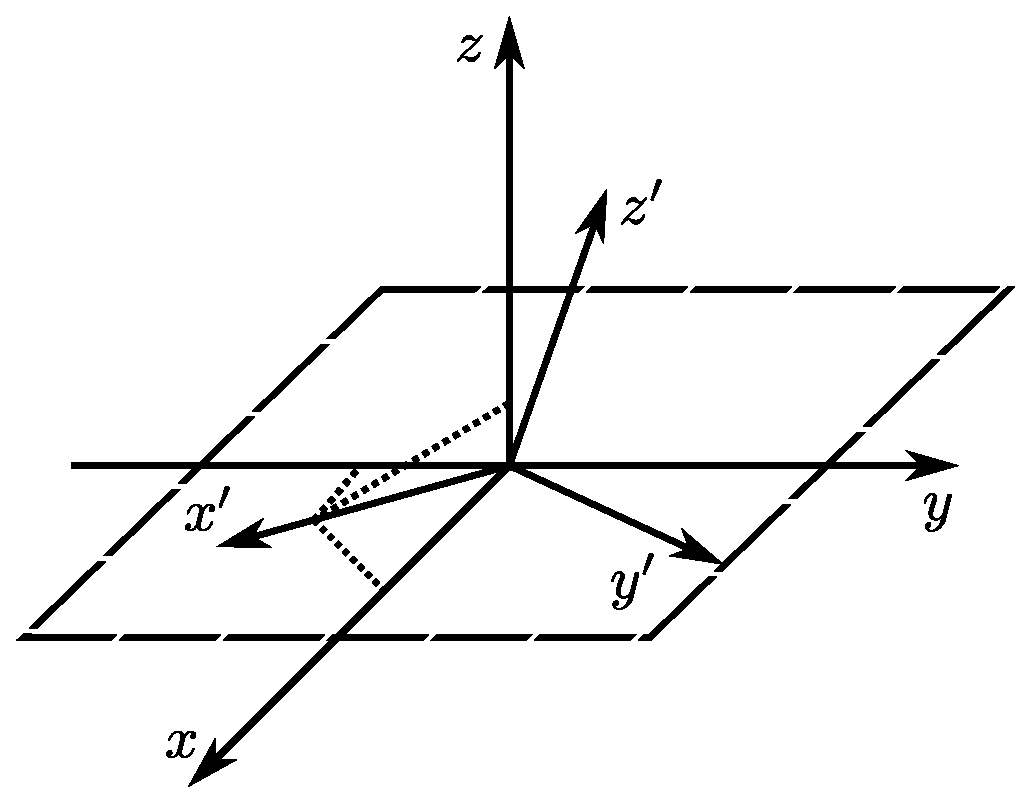
\includegraphics[width=0.5\linewidth]{figures/三维旋转坐标系}
  \caption{三维旋转坐标系}
  \label{fig:三维旋转坐标系}
\end{figure}

以$x$方向为例

\begin{equation*}
  \begin{aligned}
    x' = x \cos \alpha_1 + y \cos \beta_1 + z \cos \gamma_1
  \end{aligned}
\end{equation*}

$y$、$z$同理

\begin{equation*}
  \begin{aligned}
    y' &= y \cos \alpha_2 + y \cos \beta_2 + z \cos \gamma_2 \\
    z' &= x \cos \alpha_3 + y \cos \beta_3 + z \cos \gamma_3
  \end{aligned}
\end{equation*}

因此旋转矩阵为

\begin{equation*}
  R = 
  \begin{aligned}
    \left[
      \begin{array}{ccc}
       \cos \alpha_{1} & \cos \beta_{1} & \cos \gamma_{1}\\
       \cos \alpha_{2} & \cos \beta_{2} & \cos \gamma_{2}\\
       \cos \alpha_{3} & \cos \beta_{3} & \cos \gamma_{3}
      \end{array}
    \right ]
  \end{aligned}
\end{equation*}

则

\begin{equation*}
  \begin{aligned}
    \left[
      \begin{array}{ccc}
        x'\\
        y'\\
        z' 
      \end{array}
    \right ]
  \end{aligned}
  = R
  \begin{aligned}
    \left[
      \begin{array}{ccc}
        x\\
        y\\
        z 
      \end{array}
    \right ]
  \end{aligned}
  = 
  \begin{aligned}
    \left[
      \begin{array}{ccc}
       \cos \alpha_{1} & \cos \beta_{1} & \cos \gamma_{1}\\
       \cos \alpha_{2} & \cos \beta_{2} & \cos \gamma_{2}\\
       \cos \alpha_{3} & \cos \beta_{3} & \cos \gamma_{3}
      \end{array}
    \right ]
  \end{aligned}
  \begin{aligned}
    \left[
      \begin{array}{ccc}
        x\\
        y\\
        z 
      \end{array}
    \right ]
  \end{aligned}
\end{equation*}

\subsection{矢量分析}

Kronecker符号定义为:

\begin{equation*}
  \begin{aligned}
    \delta_{ij} =
  \end{aligned}
  \left\{
  \begin{aligned}
    & 1 && i=j \\
    & 0 && i\neq j
  \end{aligned}
  \right.
\end{equation*}

基矢之间的点乘可以表示为

\begin{equation*}
  \begin{aligned}
    \vec{e}_i \cdot \vec{e}_j = \delta_{ij}
  \end{aligned}
\end{equation*}

Levi-Civita张量定义为

\begin{equation*}
  \begin{aligned}
    \epsilon_{ijk} = 
  \end{aligned}
  \left\{
  \begin{aligned}
    & 1 && i,j,k=(1,2,3), (2,3,1),(3,1,2) \\
    & -1 && i,j,k=(3,2,1),(2,1,3),(1,3,2) \\
    & 0 && i=j\ \text{or}\ j = k \ \text{or}\ i=k
  \end{aligned}
  \right.
\end{equation*}

基矢之间的点乘可以表示为

\begin{equation*}
  \begin{aligned}
    \vec{e}_i \times \vec{e}_j = \epsilon_{ijk} \vec{e}_k
  \end{aligned}
\end{equation*}

其中运用了爱因斯坦求和转换,要对重复的字母$k$进行递归求和。

Levi-Civita张量还可以表示为

\begin{equation*}
  \begin{aligned}
    \epsilon_{ijk} = 
  \end{aligned}
  \begin{aligned}
    \left[
      \begin{array}{ccc}
       \delta_{i1} & \delta_{i2} & \delta_{i3}\\
       \delta_{j1} & \delta_{j2} & \delta_{j3}\\
       \delta_{k1} & \delta_{k2} & \delta_{k3}
      \end{array}
    \right ]
  \end{aligned}
\end{equation*}

矢量的点乘和叉乘可以表示为

\begin{equation*}
  \begin{aligned}
    & \vec{A} \cdot \vec{B} = \delta_{ij} A_i B_j = A_iB_i \\
    & \left( \vec{A} \times \vec{B} \right)_i = \epsilon_{ijk} A_j B_k
  \end{aligned}
\end{equation*}

常用的一些公式有

\begin{equation*}
  \begin{aligned}
    & \delta_{ij} \delta_{mj} = \delta_{i1} \delta_{m1} + \delta_{i2} \delta_{m2} + \delta_{i3} \delta_{m3} = \delta_{im} \\
    & \delta_{ii} = \delta_{11} + \delta_{22} + \delta_{33} = 3 \\
    & \epsilon_{ijk} \epsilon_{mnk} = \delta_{im} \delta_{jn} - \delta_{in} \delta_{jm}
  \end{aligned}
\end{equation*}

推论有

\begin{equation*}
  \begin{aligned}
    & \epsilon_{ijk} \epsilon_{mjk} = 2 \delta_{im} \\
    & \epsilon_{ijk} \epsilon_{ijk} = 6
  \end{aligned}
\end{equation*}

从此矢量的运算可以表示为

\begin{equation*}
  \begin{aligned}
    & \vec{A} + \vec{B} = \left( A_i + B_i \right) \vec{e}_i \\
    & \vec{A} \cdot \vec{B} = \left( A_i \vec{e}_i \right) \cdot \left( B_j \vec{e}_j \right) = \left( A_i B_j \right) \left( \vec{e}_i \cdot \vec{e}_j \right) = \delta_{ij} A_i B_j = A_i B_i \\
    & \vec{A} \times \vec{B} = \left( A_i \vec{e}_i \right) \times \left( B_j \vec{e}_j \right) = A_i B_j \left( \vec{e}_i \times \vec{e}_j \right) = \epsilon_{ijk} A_i B_j \vec{e}_k
  \end{aligned}
\end{equation*}

显然

\begin{equation*}
  \begin{aligned}
    \vec{A} \cdot \left( \vec{B} \times \vec{C} \right) &= \vec{A} \cdot \left( \epsilon_{ijk} B_i C_j \right) \vec{e}_k = \left( A_l \vec{e}_l \right) \left( \epsilon_{ijk} B_i C_j \vec{e}_k \right) = \delta_{lk} \epsilon_{ijk} A_l B_i C_j \\
    &= \epsilon_{ijk} A_k B_i C_j
  \end{aligned}
\end{equation*}


\begin{equation*}
  \begin{aligned}
    \vec{A} \times \left( \vec{B} \times \vec{C} \right) &= \vec{A} \times \left( \epsilon_{ijk} B_i C_j \vec{e}_k \right) = \epsilon_{mnl} A_m \left( \epsilon_{ijk} B_i C_j \vec{e}_k  \right)_n \vec{e}_l = \epsilon_{mnl} A_m \left( \epsilon_{ijn} B_i C_j \right) \vec{e}_l \\
    &= \epsilon_{mnl} \epsilon_{ijn} A_m B_i C_j \vec{e}_l = \left( \epsilon_{lmn} \epsilon_{ijn} \right) A_m B_i C_j \vec{e}_l \\
    &= \left( \delta_{li} \delta_{mj} - \delta_{lj} \delta_{mi} \right) A_m B_i C_j \vec{e}_l \\
    &= \left( A_m B_l C_m - A_m B_m C_l \right) \vec{e}_i = \left( A_m C_m \right) B_l \vec{e}_l - \left( A_m B_m \right) C_l \vec{e}_l \\
    &= \left( \vec{A} \cdot \vec{C} \right) \vec{B} - \left( \vec{A} \cdot \vec{B} \right) \vec{C}
  \end{aligned}
\end{equation*}

梯度算符可以简化为

\begin{equation*}
  \begin{aligned}
    \nabla = \vec{e}_1 \dfrac{\partial}{\partial x_1} +  \vec{e}_2 \dfrac{\partial}{\partial x_2} + \vec{e}_3 \dfrac{\partial}{\partial x_3} = \vec{e}_i \dfrac{\partial}{\partial x_i} = \vec{e}_i \partial_i 
  \end{aligned}
\end{equation*}

在直角坐标系中

\begin{equation*}
  \begin{aligned}
    \partial_i x_j = \dfrac{\partial x_j}{\partial x_i} = \delta_{ij} =  
  \end{aligned}
  \left\{
  \begin{aligned}
    & 1 && i=j \\
    & 0 && i \neq j
  \end{aligned}
  \right.
\end{equation*}

矢量的散度为

\begin{equation*}
  \begin{aligned}
    \nabla \cdot \vec{A} &= \vec{e}_i \partial_i \cdot \left( A_j \vec{e}_j \right) = \left( \vec{e}_i \cdot \vec{e}_j \right) \partial_i A_j + A_j \vec{e}_i \left( \partial_i \vec{e}_j \right) = \delta_{ij} \partial_i A_j = \partial_i A_i \\
    &= \partial_1 A_1 + \partial_2 A_2 + \partial_3 A_3 \\
    &= \dfrac{\partial A_1}{\partial x_1} + \dfrac{\partial A_2}{\partial x_2} + \dfrac{\partial A_3}{\partial x_3}   
  \end{aligned}
\end{equation*}

矢量场的旋度为

\begin{equation*}
  \begin{aligned}
    \nabla \times \vec{A} &= \left( \vec{e}_i \partial_i \right) \times \left( A_j \vec{e}_j \right) = \epsilon_{lmn} \left( \vec{e}_i \partial_i \right)_l \left( A_j \vec{e}_j \right)_m \vec{e}_n = \epsilon_{lmn} \partial_l A_m \vec{e}_n \\
    &= \left( \partial_2 A_3 - \partial_3 A_2 \right) \vec{e}_1 + \left( \partial_3 A_1 - \partial_1 A_3 \right) \vec{e}_2 + \left( \partial_1 A_2 - \partial_2 A_1 \right) \\
    &= \left[ \dfrac{\partial A_3}{\partial x_2} - \dfrac{\partial A_2}{\partial x_3}   \right] \vec{e}_1 + \left[ \dfrac{\partial A_1}{\partial x_3} - \dfrac{\partial A_3}{\partial x_1}   \right] \vec{e}_2 + \left[ \dfrac{\partial A_2}{\partial x_1} - \dfrac{\partial A_1}{\partial x_2}   \right] \vec{e}_3
  \end{aligned}
\end{equation*}

%%% Local Variables:
%%% mode: latex
%%% TeX-master: "Electro-Dynamics"
%%% End:
